Lämpöpumppujen käyttö kiinteistöjen lämmitykseen kasvattaa suosiotaan. Vuoden 2000 jälkeen on Suomeen asennettu noin 700 000 lämpöpumppua\footnote{Alle \SI{26}{\kilo\watt}}\parencite{kummu}. Lämpöpumppu saattaa olla kiinteistön ainoa lämmitysmuoto, tai se saattaa toimia toisten lämmitysjärjestelmien rinnalla. Lämpöpumpuilla voidaan korvata vanha järjestelmä, millä on vaikutusta kiinteistön lämmityksen aiheuttamaan sähkönkulutuksen luonteeseen.

\section{Lämpöpumpun toimintaperiaate}
  Lämpöpumpun eli jäähdytyskoneen toimintaperiaate on käänteinen lämpövoimakoneelle. Lämpöpumppu siirtää lämpöenergiaa viileämmästä ympäristöstä lämpimämpään.\parencite{DincerRosen}

  Lämpöpumpun perusrakenne koostuu kompressorista, lauhduttimesta, paisuntaventtiilistä ja höyrystimestä, joiden välillä kiertää kylmäaine. Järjestelmä on kuvattu kuvassa \ref{fig:hptp}. Matalassa paineessa oleva kylmäaine höyrystyy viileämmässä tilassa sijaitsevassa höyrystimessä ja vastaannottaa lämpöenergiaa. Höyrystynyt kylmäaine johdetaan lauhduttimeen ja sen paine nostetaan kompressorin avulla korkeammaksi, jolloin sen lämpötila nousee. Korkeassa paineessa ja lämpötilassa oleva kylmäaine luovuttaa lämpöenergiaa lauhduttimen välityksellä lämpimään ympäristöön, jolloin osa siitä nesteytyy. Nesteytynyt kylmäaine virtaa paisuntaventtiilin kautta takaisin höyrystimeen. Paisuntaventtiilissä kylmäaineen paine ja täten myös lämpötila laskevat.\parencite{DincerRosen}

  Höyrystimessä lämpöenergiaa siirtyy kylmäaineeseen ympäristöstä. Lämmön kuljettaminen ympäristöstä lauhduttimelle voidaan toteuttaa erilaisilla tavoilla. Suomessa yleisin tapa on käyttää ilmapuhallinta \parencite{Lahde}, joka puhaltaa ulkoilmaa höyrystimen lävitse ja jäähdyttää sitä. Tällöin kyseessä on ilmalämpöpumppu. Toinen yleinen vaihtoehto on käyttää maahan kaivettavaa tai kallioon porattavaa lämmönkeruuputkistoa. Tälläistä lämpöpumppua kutsutaan maalämpöpumpuksi. Eri sovelluskohteissa käytetään myös lukuisia muitakin lämmönlähteitä kuten ilmanvaihdon poistoilmaa, viemärivettä, lauhdevettä tai vesistöä.\parencite{DincerRosen, Lahde}

  Lauhduttimessa kylmäaineen luovuttama lämpöenergia siirretään sovelluskohteesta riippuen esimerkiksi käyttöveteen, lämmitysjärjestelmän vesikiertoon tai suoraan huoneilmaan. Teollisuudessa tuotettua energiaa voidaan käyttää esimerkiksi erilaisissa prosesseissa\parencite{Setala}. Sovelluskohde määrää lauhduttimelta vaadittavan lämpötilan. Järjetelmiä saatetaan kutsua erilaisilla nimillä riippuen siitä, mihin tuotetteua energiaa käytetään. Mikäli tuotettulla energialla lämmitetään käyttövettä tai lämmitysjärjetelmän kiertovettä, kutsutaan laitetta Ilma--vesilämpöpumpuksi.\parencite{Lahde}

  Lämpöpumpun lämpökerroin, eli COP\footnote{Coefficient Of Performance} määritellään lämpöpumpun tuottaman lämpötehon ja sen kuluttaman sähkötehon suhteena.
  \begin{displaymath}
      \textrm{COP} = \frac{\dot{Q}}{\dot{P}}
  \end{displaymath}
  Normaali lämpöpumppujen lämpökerroin vaihtelee välillä 2 -- 5. Lämpökerroin ja sen vaihtelu riippuvat paljolti lämmön lähteestä: maalämpöpumpuilla on yleensä korkeampi lämpökerroin kuin ilmalämpöpumppuilla.\parencite{DincerRosen}

  \begin{figure}
    \centering
    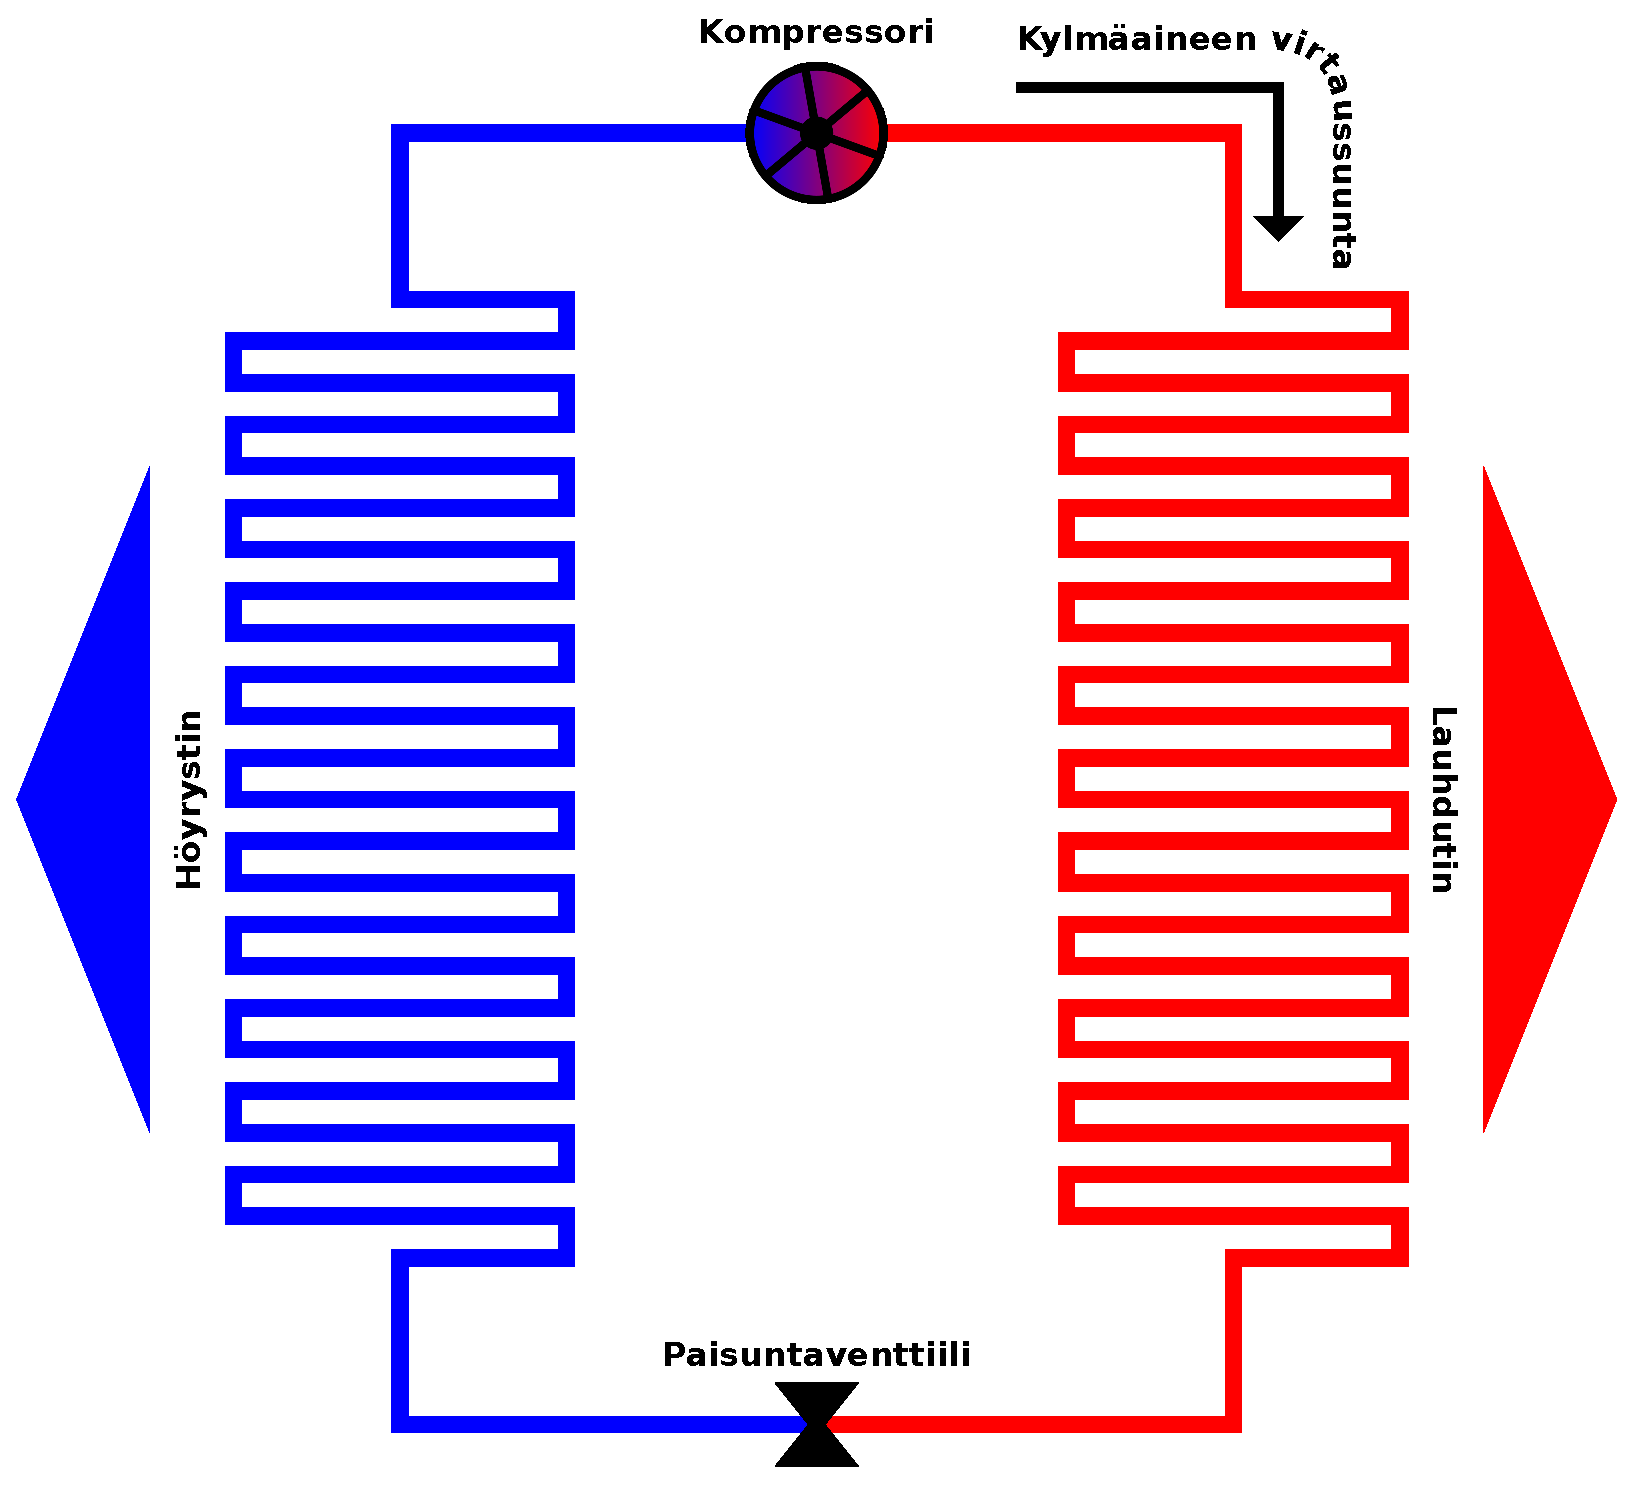
\includegraphics[width=0.5\textwidth]{figures/hp}
    \caption{Lämpöpumpun toimintaperiaate}
    \label{fig:hptp}
  \end{figure}

  Lämpöpumput käyttävät sähköenergiaa lämmön siirtämiseen viileämmästä lämpövarastosta lämpimämpään. Käytetystä sähköenergiasta valtaosa kuluu paineen tuottamiseen kompressorilla, mikä ylläpitää energiaa tuottavaa työkiertoa. Kompressorin lisäksi sähköä kuluu pienempiä määriä vaikkapa lämpöpumpun ohjaukseen, lämmitysjärjestelmän kiertovesipumpun käyttämiseen tai puhaltimen käyttämiseen. Mikäli lämpöpumpun teho on mitoitettu pienemmäksi kuin suurin vaadittu lämmitysteho\footnote{osatehomitoitus}, voidaan tehojen erotus tuottaa tarvittaessa lämpöpumpun yhteyteen asennettavilla sähkövastuksilla. Tälläinen ratkaisu lisää huomattavasti järjestelmän sähkönkulutusta suurimman energiantarpeen aikana, jolloin sähköä käytetään muutenkin enemmän.

  Lämpöpumpuissa kompressorin pyörittämiseen käytetään sähkömoottoria. Vanhemmissa lämpöpumpuissa moottori on useimmiten verkkojännitteeseen kytketty oikosulkumoottori, joka voidaan tarvittaessa varustaa käynnistyksen ohjauksella eli pehmokäynnistimellä. Nykyaikaisemmassa ratkaisuissa oikosulkumoottoria käytetään taajuusmuuttajan avulla.

  \section{Oikosulkumoottori}
    Yleisin tapa pyörittää lämpöpumpun kompressoria on käyttää suoraan verkkojännitteeseen kytkettyä oikosulkumoottoria. Kompressorin tehoa ei voida säädellä, vaan käydessään se tuottaa aina vakiotehon. Tälläisen lämpöpumpun tehoa säädetään kytkemällä kompressoria päälle ja pois. Kompressori kytkeytyy päälle, kun lämmitettävän ympäristön, esimerkiksi lämminvesivaraajan tai sisäilman, lämpötila laskee tietyn rajan alapuolelle. Kun lämmitettävän ympäristön lämpötila on noussut tarpeeksi, sammutetaan kompressori.

    Tärkeimmät kompressorin käyntijaksojen pituuteen vaikuttavat tekijät ovat lämmitettävän ympäristön haluttu lämpötila, lämmönlähteen lämpötila ja kompressorin teho. Kotitalousköytössä kompressoreiden tehot ovat yleensä muutamia kilowatteja\footnote{etsi tarkempi tieto}.

    Mikäli oikosulkumoottorin käynnistysvirtaa ei mitenkään rajoiteta, on se tyypillisesti 4 -- 8 kertainen moottorin nimellisvirtaan nähden. Täten myös moottorin sähköverkosta ottama teho on suuri.\parencite{rautiainen} Käynnistyksen jälkeen moottorin ottama virta laskee nimellisarvoonsa ja moottori ottaa verkosta nimellistehonsa.

  \section{Oikosulkumoottori virranrajoittimella}

  \section{Inventterikäyttö}
